\documentclass{article}

\usepackage{graphicx}
\usepackage{tikz}
\usepackage{tikzsymbols}
\usetikzlibrary{calc,patterns,shapes.geometric}
\pagestyle{empty}
\usepackage[margin=0pt]{geometry}
\geometry{papersize={14in,12in}}

\def\centerarc[#1](#2)(#3:#4:#5){\draw[#1] ($(#2)+({#5*cos(#3)},{#5*sin(#3)})$) arc (#3:#4:#5);}

\begin{document}
	\begin{figure}
		\centering
		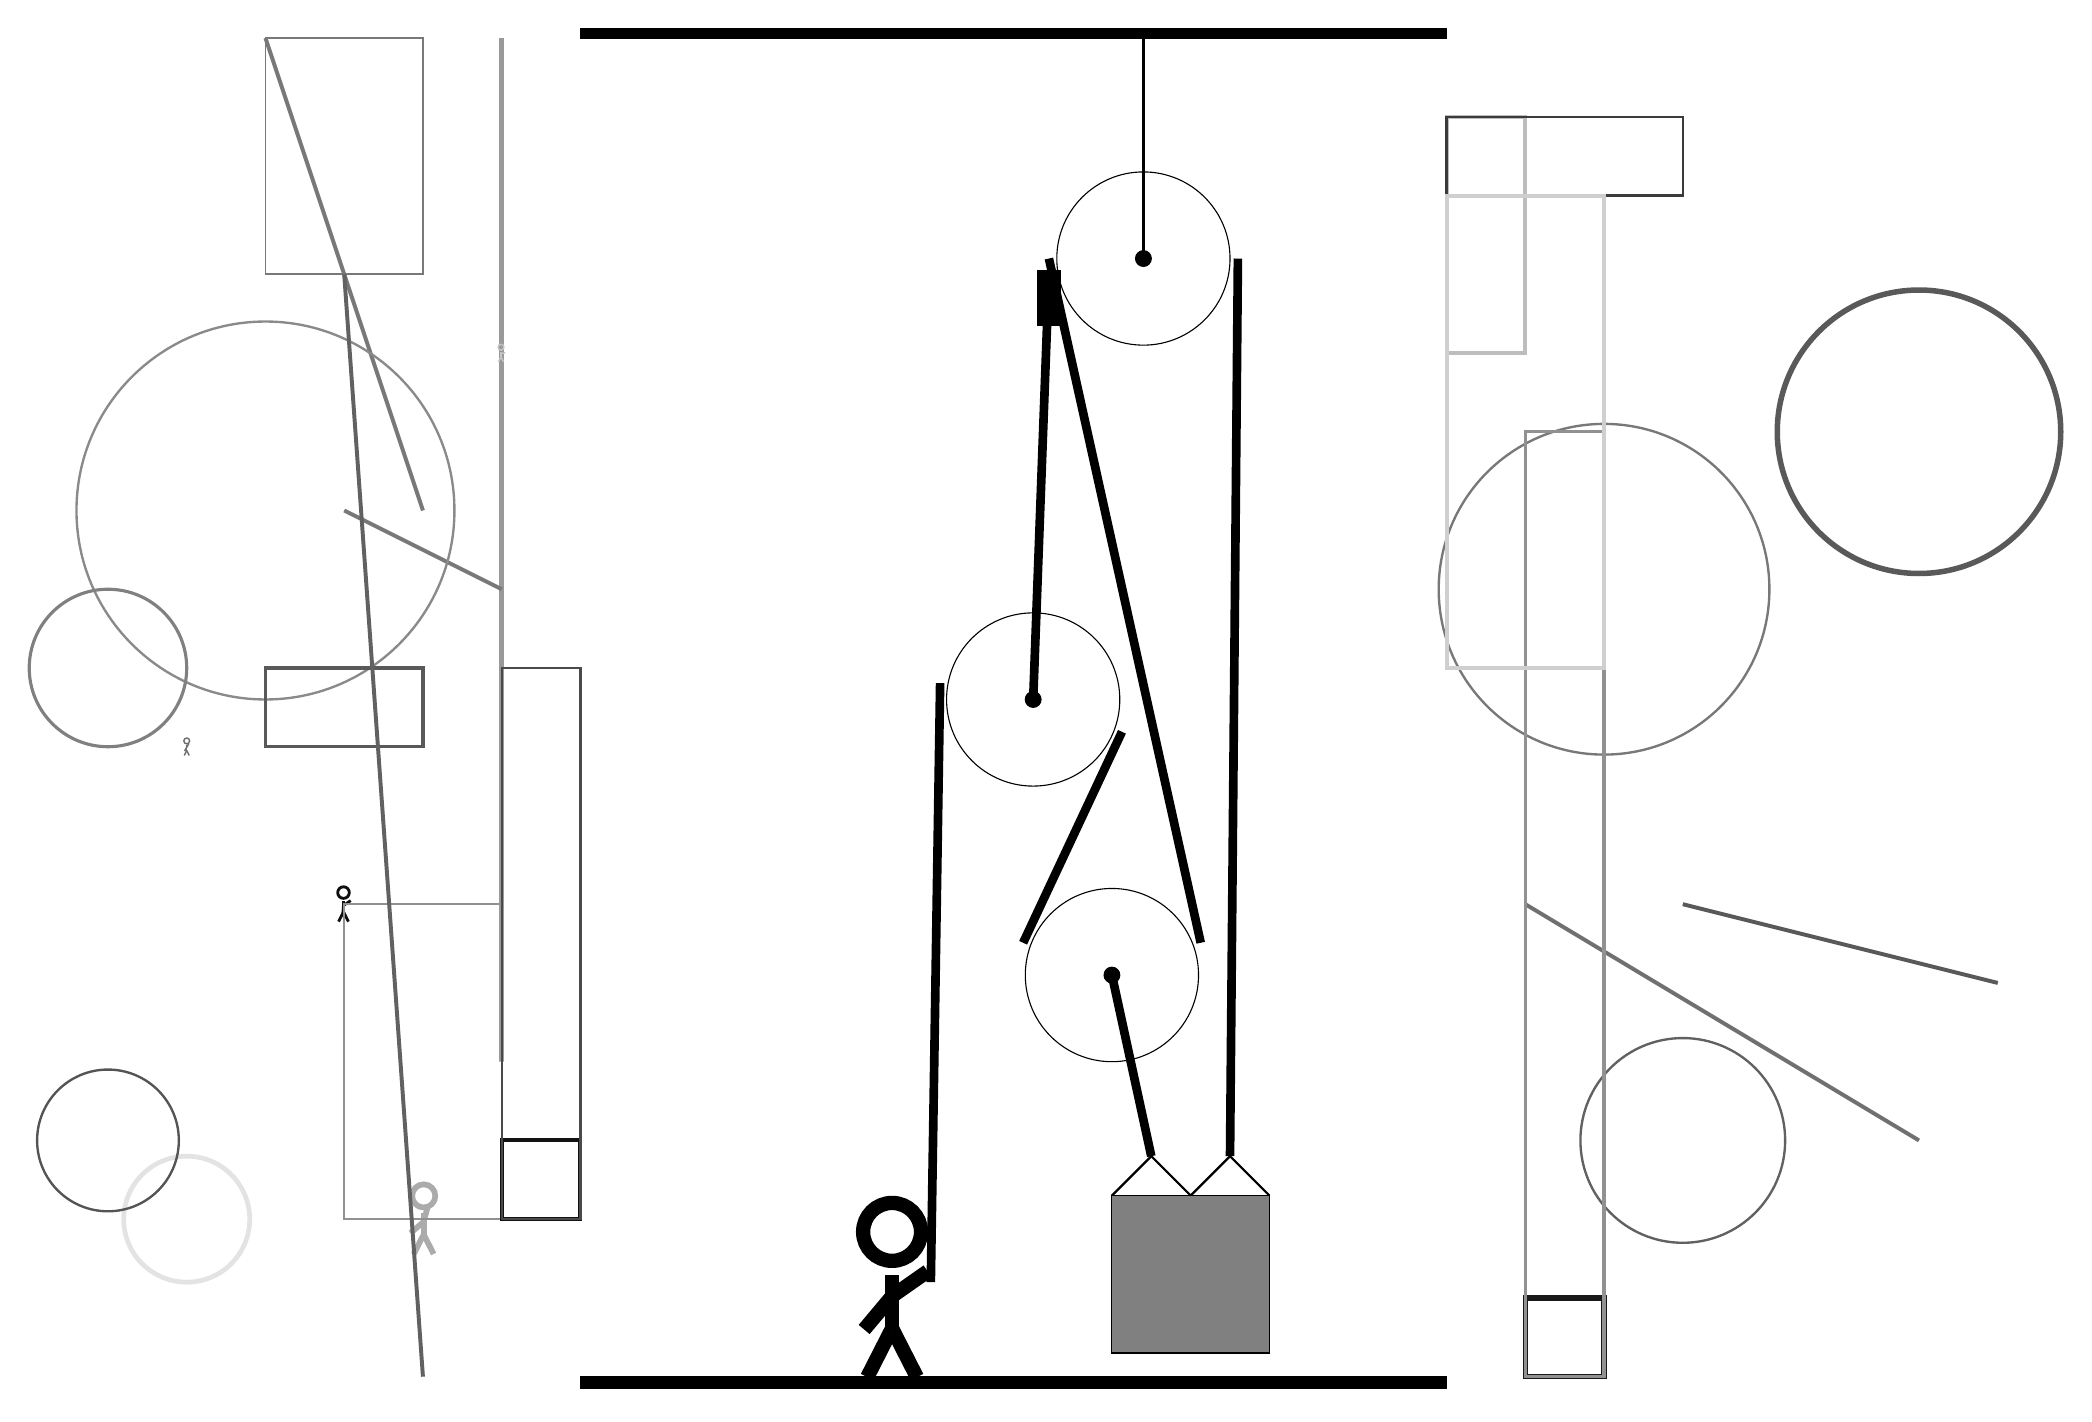
\begin{tikzpicture}
			%%%%% START %%%%%
			
			\draw[fill=black] (-6, 14) rectangle (5, 14.125);
			
			\draw (-0.25, 5.6) circle (1.1);
			\draw[fill=black] (-0.25, 5.6) circle (0.1);
			
			\draw (0.75, 2.1) circle (1.1);
			\draw[fill=black] (0.75, 2.1) circle (0.1);
			
			\draw (1.15, 11.2) circle (1.1);
			\draw[fill=black] (1.15, 11.2) circle (0.1);
			\draw[very thick] (1.15, 11.2) -- (1.15, 14);
			
			\draw [line width=0.6mm, color=black!11](-11, -1) circle (0.8);
			
			\draw[line width=0.6mm, color=black!40] (-7, 1) rectangle (-7, 14);
			\draw[line width=0.5mm, color=black!53](-9, 8) -- (-7, 7);
			\draw [line width=0.3mm, color=black!53](7, 7) circle (2.1);
			\draw[line width=0.2mm, color=black!53] (-8, 11) rectangle (-10, 14);
			\draw[line width=0.5mm, color=black!75] (-7, 1) rectangle (-7, 1);
			\node[line width=0.5mm, color=black!94] at (-9, 3) {\Strichmaxerl[2][86][34]};
			\draw[line width=0.5mm, color=black!65](8, 3) -- (12, 2);
			\draw[line width=0.5mm, color=black!53](-8, 8) -- (-10, 14);
			\node[line width=0.6mm, color=black!23] at (-7, 10) {\Strichmaxerl[1][86][13]};
			\draw [line width=0.7mm, color=black!65](11, 9) circle (1.8);
			\node[line width=0.2mm, color=black!33] at (-8, -1) {\Strichmaxerl[4][41][75]};
			\draw[line width=0.5mm, color=black!26] (6, 10) rectangle (5, 13);
			
			\draw[line width=0.5mm, color=black!56](6, 3) -- (11, 0);
			\draw[line width=0.2mm, color=black!43] (-7, -1) rectangle (-9, 3);
			\draw [line width=0.3mm, color=black!62](8, 0) circle (1.3);
			
			\draw[line width=0.3mm, color=black!77] (5, 12) rectangle (8, 13);
			\draw [line width=0.3mm, color=black!46](-10, 8) circle (2.4);
			\draw[line width=0.5mm, color=black!93] (-7, 0) rectangle (-6, -1);
			\draw[line width=0.3mm, color=black!71] (-7, 6) rectangle (-6, -1);
			\draw [line width=0.4mm, color=black!50](-12, 6) circle (1.0);
			
			\draw[line width=0.7mm, color=black!90] (7, -2) rectangle (6, -3);
			\draw[line width=0.4mm, color=black!43] (6, -3) rectangle (7, 9);
			\draw[line width=0.4mm, color=black!65] (-8, 5) rectangle (-10, 6);
			\node[line width=0.5mm, color=black!57] at (-11, 5) {\Strichmaxerl[1][59][61]};
			
			\draw[line width=0.5mm, color=black!62](-9, 11) -- (-8, -3);
			\draw [line width=0.3mm, color=black!67](-12, 0) circle (0.9);
			\draw[line width=0.5mm, color=black!19] (7, 12) rectangle (5, 6);
			
			\draw [line width=0.6mm, color=black!81](-11, 13) circle (0.0);
			
			\draw[thick]  (0.75, -0.7) -- (1.25, -0.2) -- (1.75, -0.7) -- (2.25, -0.2) -- (2.75, -0.7);
			\draw[fill=black!50] (0.75, -0.7) rectangle (2.75, -2.7);
			
			\draw[line width=1.1mm] (-0.25, 5.6) -- (-0.05, 11.0);
			\draw[line width=1.1mm, fill=black](-0.15, 10.4) rectangle (0.05, 11.0);
			\draw[line width=1.1mm] (-1.55, -1.8) -- (-1.4318, 5.8083);
			\centerarc[line width=1.1mm](-0.25, 5.6)(-20:170:1.2000000000000002);
			\draw[line width=1.1mm] (0.8776, 5.1896) -- (-0.3776, 2.5104);
			\centerarc[line width=1.1mm](0.75, 2.1)(160:380:1.2000000000000002);
			\draw[line width=1.1mm] (1.8776, 2.5104) -- (-0.05, 11.2);
			\draw[line width=1.1mm](0.75, 2.1) -- (1.25, -0.2);
			\centerarc[line width=1.1mm](1.15, 11.2)(0:180:1.2000000000000002);
			\draw[line width=1.1mm] (2.35, 11.2) -- (2.25, -0.2);
			
			\node at (-2, -1.9) {\Strichmaxerl[10][50][35]};
			
			\draw[fill=black] (-6, -3) rectangle (5, -3.15);
			
			%%%%% END %%%%%
		\end{tikzpicture}
	\end{figure}	
\end{document}